\documentclass[12pt]{article}

\usepackage{tikz} % картинки в tikz
\usepackage{microtype} % свешивание пунктуации
\usepackage{array} % для столбцов фиксированной ширины
\usepackage{comment} % для комментирования целых окружений
\usepackage{indentfirst} % отступ в первом параграфе

\usepackage{sectsty} % для центрирования названий частей
\allsectionsfont{\centering}

\usepackage{amsmath, amssymb, amsthm, amsfonts} % куча стандартных математических плюшек

\usepackage[top=2cm, left=1cm, right=1cm, bottom=2cm]{geometry} % размер текста на странице
\usepackage{lastpage} % чтобы узнать номер последней страницы
 
\usepackage{enumitem} % дополнительные плюшки для списков
%  например \begin{enumerate}[resume] позволяет продолжить нумерацию в новом списке

\usepackage{caption} % подписи к рисункам
\usepackage{hyperref} % гиперссылки
\usepackage{multicol} % текст в несколько столбцов


\usepackage{fancyhdr} % весёлые колонтитулы
\pagestyle{fancy}
\lhead{Введение в глубокое обучение, ЭМИТ, РАНХ}
\chead{}
\rhead{2022-04-01}
\lfoot{Вариант $\pi$}
\cfoot{}
\rfoot{Паниковать запрещается!}
\renewcommand{\headrulewidth}{0.4pt}
\renewcommand{\footrulewidth}{0.4pt}

\usepackage{ifthen} % для написания условий

\usepackage{todonotes} % для вставки в документ заметок о том, что осталось сделать
% \todo{Здесь надо коэффициенты исправить}
% \missingfigure{Здесь будет Последний день Помпеи}
% \listoftodos --- печатает все поставленные \todo'шки


% более красивые таблицы
\usepackage{booktabs}
% заповеди из докупентации:
% 1. Не используйте вертикальные линни
% 2. Не используйте двойные линии
% 3. Единицы измерения - в шапку таблицы
% 4. Не сокращайте .1 вместо 0.1
% 5. Повторяющееся значение повторяйте, а не говорите "то же"


\usepackage{fontspec}
\usepackage{polyglossia}

\setmainlanguage{russian}
\setotherlanguages{english}

% download "Linux Libertine" fonts:
% http://www.linuxlibertine.org/index.php?id=91&L=1
\setmainfont{Linux Libertine O} % or Helvetica, Arial, Cambria
% why do we need \newfontfamily:
% http://tex.stackexchange.com/questions/91507/
\newfontfamily{\cyrillicfonttt}{Linux Libertine O}

% Математические шрифты 
\usepackage{unicode-math}     
\setmathfont[math-style=upright]{[Neo Euler.otf]} 

\AddEnumerateCounter{\asbuk}{\russian@alph}{щ} % для списков с русскими буквами
\setlist[enumerate, 2]{label=\asbuk*),ref=\asbuk*}



% мои цвета https://www.artlebedev.ru/colors/
\definecolor{titleblue}{rgb}{0.2,0.4,0.6} 
\definecolor{blue}{rgb}{0.2,0.4,0.6} 
\definecolor{red}{rgb}{1,0,0.2} 
\definecolor{green}{rgb}{0,0.6,0} 
\definecolor{purp}{rgb}{0.4,0,0.8} 

% цвета из geogebra 
\definecolor{litebrown}{rgb}{0.6,0.2,0}
\definecolor{darkbrown}{rgb}{0.75,0.75,0.75}

% Гиперссылки
\usepackage{xcolor}   % разные цвета

\usepackage{hyperref}
\hypersetup{
    unicode=true,           % позволяет использовать юникодные символы
    colorlinks=true,        % true - цветные ссылки
    urlcolor=blue,          % цвет ссылки на url
    linkcolor=black,          % внутренние ссылки
    citecolor=green,        % на библиографию
    breaklinks              % если ссылка не умещается в одну строку, разбивать её на две части?
}

% эпиграфы
\usepackage{epigraph}
\setlength\epigraphwidth{.5\textwidth}
\setlength\epigraphrule{0pt}

% Математические операторы первой необходимости:
\DeclareMathOperator{\sgn}{sign}
\DeclareMathOperator*{\argmin}{arg\,min}
\DeclareMathOperator*{\argmax}{arg\,max}
\DeclareMathOperator{\Cov}{Cov}
\DeclareMathOperator{\Var}{Var}
\DeclareMathOperator{\Corr}{Corr}
\DeclareMathOperator{\E}{\mathop{E}}
\DeclareMathOperator{\Med}{Med}
\DeclareMathOperator{\Mod}{Mod}
\DeclareMathOperator*{\plim}{plim}

\DeclareMathOperator{\logloss}{logloss}
\DeclareMathOperator{\softmax}{softmax}

\DeclareMathOperator{\tr}{tr}

% команды пореже
\newcommand{\const}{\mathrm{const}}  % const прямым начертанием
\newcommand{\iid}{\sim i.\,i.\,d.}  % ну вы поняли...
\newcommand{\fr}[2]{\ensuremath{^{#1}/_{#2}}}   % особая дробь
\newcommand{\ind}[1]{\mathbbm{1}_{\{#1\}}} % Индикатор события
\newcommand{\dx}[1]{\,\mathrm{d}#1} % для интеграла: маленький отступ и прямая d

% одеваем шапки на частые штуки
\def \hb{\hat{\beta}}
\def \hs{\hat{s}}
\def \hy{\hat{y}}
\def \hY{\hat{Y}}
\def \he{\hat{\varepsilon}}
\def \hVar{\widehat{\Var}}
\def \hCorr{\widehat{\Corr}}
\def \hCov{\widehat{\Cov}}

% Греческие буквы
\def \a{\alpha}
\def \b{\beta}
\def \t{\tau}
\def \dt{\delta}
\def \e{\varepsilon}
\def \ga{\gamma}
\def \kp{\varkappa}
\def \la{\lambda}
\def \sg{\sigma}
\def \tt{\theta}
\def \Dt{\Delta}
\def \La{\Lambda}
\def \Sg{\Sigma}
\def \Tt{\Theta}
\def \Om{\Omega}
\def \om{\omega}

% Готика
\def \mA{\mathcal{A}}
\def \mB{\mathcal{B}}
\def \mC{\mathcal{C}}
\def \mE{\mathcal{E}}
\def \mF{\mathcal{F}}
\def \mH{\mathcal{H}}
\def \mL{\mathcal{L}}
\def \mN{\mathcal{N}}
\def \mU{\mathcal{U}}
\def \mV{\mathcal{V}}
\def \mW{\mathcal{W}}

% Жирные буквы
\def \mbb{\mathbb}
\def \RR{\mbb R}
\def \NN{\mbb N}
\def \ZZ{\mbb Z}
\def \PP{\mbb{P}}
\def \QQ{\mbb Q}

\def \putyourname{\fbox{
    \begin{minipage}{42em}
      Фамилия, имя, номер группы:\vspace*{3ex}\par
      \noindent\dotfill\vspace{2mm}
    \end{minipage}
  }
}

\def \checktable{

    \vspace{5pt}
    Табличка для проверяющих работу:

\vspace{5pt}

    \begin{tabular}{|m{2cm}|m{1cm}|m{1cm}|m{1cm}|m{1cm}|m{1cm}|m{2cm}|}
\toprule
        Тест & 1 &  2 & 3 & 4 & 5 & Итого \\
\midrule
        &  &  & & & & \\
        &  &  & & & & \\
 \bottomrule
\end{tabular}
}


\def \testtable{

\vspace{5pt}
    Внесите сюда ответы на тест:

\vspace{5pt}

\begin{tabular}{|m{2cm}|m{0.6cm}|m{0.6cm}|m{0.6cm}|m{0.6cm}|m{0.6cm}|m{0.6cm}|m{0.6cm}|m{0.6cm}|m{0.6cm}|m{0.6cm}|}
\toprule
        Вопрос & 1 &  2 & 3 & 4 & 5 & 6 & 7 & 8 & 9 & 10 \\
\midrule
        Ответ &  &  & & & & & & & & \\
 \bottomrule
\end{tabular}
}


% [1][3] 1 = one argument, 3 = value if missing
% эта магия создаёт окружение answerlist
% именно в окружении answerlist записаны варианты ответов в подключаемых exerciseXX
% просто \begin{answerlist} сделает ответы в три столбца
% если ответы длинные, то надо в них руками сделать
% \begin{answerlist}[1] чтобы они шли в один столбец
\newenvironment{answerlist}[1][3]{
\begin{multicols}{#1}

\begin{enumerate}[label=\fbox{\emph{\Alph*}},ref=\emph{\alph*}]
}
{
\item Нет верного ответа.
\end{enumerate}
\end{multicols}
}

% BB: unicol version. don't know why \ifthenelse fails in second part of new-env
\newenvironment{answerlistu}{
\begin{enumerate}[label=\fbox{\emph{\Alph*}},ref=\emph{\alph*}]
}
{
\item Нет верного ответа.
\end{enumerate}
}


\excludecomment{solution} % without solutions

\theoremstyle{definition}
\newtheorem{question}{Вопрос}

\usepackage{tikzlings}
\usepackage{tikzducks}
\usepackage{float}

\usepackage{alltt}

\begin{document}

\putyourname

% \testtable

% \checktable

\epigraph{Чем больше преград, тем жёстче подход. \\ Я не вижу берегов, мне нужен мой запретный плод.}{\textit{The Hatters, Shoot Me (2021)}}

Это нулевой вариант мидтёрма. Он нужен для того, чтобы его формат не стал для вас сюрпризом. Работа будет состоять из трёх частей:  тестовая, задачи и ответы на открытые вопросы. Списывание будет карается обнулением работы. \textbf{Разрешается использовать шпаргалку формата А4, исписанную с двух сторон. Передача шпаргалки другим людям запрещена.} Удачи!

\section*{Часть первая: тестовая} 

Дайте ответ на $10$ тестовых вопросов. Каждый вопрос стоит $3$ балла. Никакие дополнительные пояснений в этой части работы от вас не требуются. В части вопросов верными могут быть несколько ответов. За неправильные ответы вы не получаете никаких штрафов. 

\begin{question}
Какие из следующих функций активации могут привести к затуханию градиентов и параличу глубокой нейронной сети?
\begin{answerlist}
  \item ReLU
  \item Tanh
  \item Leaky ReLU
  \item Сигмоида
  \item Mish
\end{answerlist}
\end{question}

\begin{solution}
\begin{answerlist}
  \item Bad answer :(
  \item Good answer :)
  \item Bad answer :(
  \item Good answer :)
  \item Bad answer :(
\end{answerlist}
\end{solution}

\begin{question}
Какие из следующих техник могут быть использованы для аугментации данных в задаче распознавания изображений? 
    \begin{answerlist}
      \item Зеркальное отражение
      \item Случайное обрезание
      \item Случайные повороты
      \item Смена цветовой гаммы
      \item Масштабирование (зум)
    \end{answerlist}
\end{question}

\begin{solution}
    \begin{answerlist}
      \item Good answer :)
      \item Good answer :)
      \item Good answer :)
      \item Good answer :)
      \item Good answer :)
    \end{answerlist}
\end{solution}

\begin{question}
У нас есть полносвязная сеть с тремя слоями. На каком-то из наблюдений, на последнем слое нейросеть выплёвывает вектор $[0.3, 0.3, 0.3].$ К нему применяется некоторая функция активации. Каким будет результат её применения, если мы решаем задачу классификации на три класса? 
\begin{answerlist}
  \item  $[0.5, 0.5, 0.5]$
  \item  $[1, 0, 0]$
  \item  $[0.2, 0.5, 0.3]$
  \item  $[0, 0, 0]$
  \item  $[0.3, 0.3, 0.3]$
\end{answerlist}
\end{question}

\begin{solution}
\begin{answerlist}
  \item Bad answer :(
  \item Bad answer :(
  \item Bad answer :(
  \item Bad answer :(
  \item Bad answer :(
\end{answerlist}
\end{solution}


\begin{question}
Какой сложностью по времени обладает алгоритм обратного распространения ошибки? Под $m$ тут имеется в виду глубина сети.
\begin{answerlist}
  \item $O(m!)$
  \item $O(m^2)$
  \item $O(m)$
  \item $O(m\ln m)$
  \item $O(\ln m)$
\end{answerlist}
\end{question}

\begin{solution}
\begin{answerlist}
  \item Bad answer :(
  \item Bad answer :(
  \item Good answer :)
  \item Bad answer :(
  \item Bad answer :(
\end{answerlist}
\end{solution}

\newpage 

\begin{question}
Предположим, что на первом слое нейронной сети у нас есть $5$ свёрток размера $7 \times 7$ с дополнением нулями (zero padding) и сдвигом равным единице (stride). На вход подаётся изображение размера $224 \times 224 \times 3$. Какого размера будет тензор, который пройдёт через этот слой.  
\begin{answerlist}
  \item $217 \times 217 \times 3$
  \item $217 \times 217 \times 8$
  \item $220 \times 220 \times 5$
  \item $224 \times 224 \times 5$
  \item $218 \times 218 \times 5$
\end{answerlist}
\end{question}

\begin{solution}
\begin{answerlist}
  \item Bad answer :(
  \item Bad answer :(
  \item Bad answer :(
  \item Bad answer :(
  \item Good answer :)
\end{answerlist}
\end{solution}
 
 
\begin{question}
Выберите все верные утверждения
\begin{answerlist}
  \item Нормализация по батчам --- это новый способ реализации дропаута.
  \item Нормализация по батчам ускоряет обучение
  \item В нормализации по батчам мы усредняем столбцы матрицы (признаки). 
  \item Нормализация по батчам может конфликтовать с дропаутом
  \item Нормализация по батчам --- это нелинейная трансформация данных, которая делает среднее нулевым. 
\end{answerlist}
\end{question}
\begin{solution}
\begin{answerlist}
  \item Bad answer :(
  \item Good answer :)
  \item Bad answer :(
  \item Good answer :)
  \item Bad answer :(
\end{answerlist}
\end{solution}


\begin{question}
Вы обучаете свёрточную нейронную сеть на ImageNet. Для этого вы собираетесь использовать градиентный спуск. Какие из перечисленных утверждений являются правдой? Под скоростью тут имеется в виду время в минутах. 
\begin{answerlist}
  \item Возможно, SGD по одному наблюдению сойдётся быстрее, чем SGD по мини-батчам.
  \item Возможно, что обычный градиентный спуск сойдётся быстрее, чем Adam. 
  \item Возможно, SGD по мини-батчам сойдётся быстрее обычного градиентного~спуска.
  \item Возможно, что Adam сойдётся быстрее, чем обычный градиентный спуск.
  \item Возможно, SGD по мини-батчам сойдётся быстрее, чем SGD по одному наблюдению.
\end{answerlist}
\end{question}

\begin{solution}
\begin{answerlist}
  \item Good answer :)
  \item Bad answer :(
  \item Good answer :)
  \item Good answer :)
  \item Good answer :)
\end{answerlist}
\end{solution}


\begin{question}
Предположим, что у нас есть глубокая нейронная сеть обученная для классификации на ImageNet. Мы хотим научиться классифицировать автомобили $10$ разных типов: спорткары, траки, минивэны и т.д. В нашем расапоряжении есть выборка из $300$ картинок. Выберите все способы обучить модель, которые дадут хорошее качество классификации. 
\begin{answerlist}
  \item Обучение свёрточной нейросети с нуля на $300$ изображениях.
  \item Заморозить в большой сети все слои и доучить для решения нашей задачи только последний. 
  \item Случайно инициализировать в большой сети все веса и обучить её для нашей задачи. 
  \item Заморозить в большой сети случайную половину слоёв, а вторую половину доучить.
  \item Заморозить в большой сети все слои и доучить для решения нашей задачи два последних. 
\end{answerlist}
\end{question}

\begin{solution}
\begin{answerlist}
  \item Bad answer :(
  \item Good answer :)
  \item Bad answer :(
  \item Bad answer :(
  \item Good answer :)
\end{answerlist}
\end{solution}

\newpage 

\begin{question}
Выберите все верные утверждения о современных свёрточных архитектурах. 
\begin{answerlist}
  \item ResNet это обычная свёрточная сетка, но увеличенная в тысячу раз. 
  \item VGG и ResNet показывают сопоставимые результаты на ImageNet.
  \item Ключевой элемент ResNet это skip-connection, который добавляется чтобы исправлять ошибки предыдущих слоёв.
  \item В современных архитектурах отказались от идеи свёрточного слоя.
  \item Сделать одну свёртку размера $5\times5$ предпочтительнее, чем сделать друг за другом две свёртки размера $3\times3$.
\end{answerlist}
\end{question}

\begin{solution}
\begin{answerlist}
  \item Bad answer :(
  \item Good answer :)
  \item Bad answer :(
  \item Good answer :)
  \item Bad answer :(
\end{answerlist}
\end{solution}
 
\begin{question}
Выберите все хорошие практики, используемые при организации DL-экспериментов.
\begin{answerlist}
  \item Делать по одному изменению за раз
  \item Логировать все эксперименты
  \item Тестировать на одном батче
  \item Использовать проверенные временем архитектуры
  \item Никогда не использовать нормализацию по батчам
\end{answerlist}
\end{question}

\begin{solution}
\begin{answerlist}
  \item Bad answer :(
  \item Good answer :)
  \item Bad answer :(
  \item Good answer :)
  \item Bad answer :(
\end{answerlist}
\end{solution}
 
 
 
\newpage 

\section*{Часть вторая: задачки}

Все ответы должны быть обоснованы. Решения должны быть прописаны для каждого пункта. Рисунки должны быть чёткими и понятными. Все линии должны быть подписаны. За решение каждой задачи можно получить $8$ баллов.

\begin{question} Рассмотрим следующие функции активации: SoftPlus и ReLU: 
    \[
    ReLU(z) = \max(0, z) \qquad SoftPlus(z) = \ln(1 + e^z).
    \]
    
    \begin{enumerate}
        \item В современных нейронных сетях SoftPlus в отличие от ReLU практически не используется. Перечислите основные приемущества ReLU перед SoftPlus. 
        \item Выпишите уравнения для шага обратного распространения для обеих функций активации. 
        \item Как взаимосвязаны SoftPlus и сигмоида? Может ли привести использование SoftPlus к параличу нейронной сети? 
        \item ReLU потенциально может занулить выход из слоя нейроной сети. Как на практике решают эту проблему? 
    \end{enumerate} 
\end{question}


\newpage 


\begin{question}
У Мирона есть картинка размера $3 \times 4$ и свёртка размера $3 \times 3$
    \begin{figure}[H]
    \begin{minipage}{0.49\linewidth} 
        \centering
        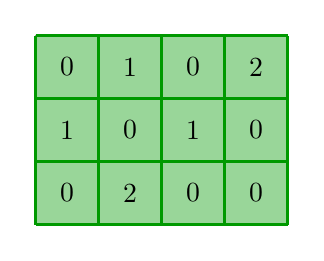
\begin{tikzpicture}[scale=.8,every node/.style={minimum size=1cm}, on grid]
                \draw[fill=green,opacity=0.4] (0,0) rectangle (4,3);
                \draw[draw=green,thick] (0,0) grid (4,3);
                \node (00) at (0.5,2.5) {0};
                \node (01) at (1.5,2.5) {1};
                \node (02) at (2.5,2.5) {0};
                \node (03) at (3.5,2.5) {2};
                
                \node (10) at (0.5,1.5) {1};
                \node (11) at (1.5,1.5) {0};
                \node (12) at (2.5,1.5) {1};
                \node (13) at (3.5,1.5) {0};
                
                \node (20) at (0.5,0.5) {0};
                \node (21) at (1.5,0.5) {2};
                \node (22) at (2.5,0.5) {0};
                \node (23) at (3.5,0.5) {0};
        \end{tikzpicture}
        \\ Картинка
    \end{minipage} 
    \hfill
    \begin{minipage}{0.49\linewidth} 
        \centering
        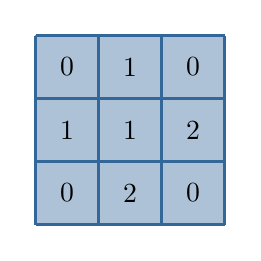
\begin{tikzpicture}[scale=.8,every node/.style={minimum size=1cm}, on grid]
                \draw[fill=blue,opacity=0.4] (0,0) rectangle (3,3);
                \draw[draw=blue,thick] (0,0) grid (3,3);
                \node (00) at (0.5,2.5) {0};
                \node (01) at (1.5,2.5) {1};
                \node (02) at (2.5,2.5) {0};
                \node (10) at (0.5,1.5) {1};
                \node (11) at (1.5,1.5) {1};
                \node (12) at (2.5,1.5) {2};
                \node (20) at (0.5,0.5) {0};
                \node (21) at (1.5,0.5) {2};
                \node (22) at (2.5,0.5) {0};
        \end{tikzpicture}
        \\ Свёртка
    \end{minipage} 
    \end{figure}
    \begin{enumerate} 
        \item Пусть используется дополнение нулями (zero padding). Найдите результат применения свёртки к исходной картинке.
        \item Пусть при свёртке не используется никаких дополнений. Найдите результат применения свёртки к исходной картинке.
    \end{enumerate} 
\end{question}

\vspace{4cm} 

\begin{question}
Свёрточная сеть состоит из $N$ слоёв. Каждый слой состоит из свёртки с ядром размера $3 \times 3,$ сигмоиды и max-pooling размера $2 \times 2$. Входное изображение имеет размер $512 \times 512.$ 
    \begin{enumerate} 
        \item Какого размера будет выход первого слоя?
        \item Какого размера будет выход второго слоя? 
        \item Каким должно быть $N$, чтобы на выходе получилось изображение размера $1 \times 1$? Каким при этом $N$ будет поле обзора (receptive field)? 
    \end{enumerate} 
\end{question}


\newpage 

\begin{question}
    Пусть $A, X$ --- матрицы размера $n \times n$. Для следующей задачи оптимизации найдите ее множество решений и оптимальное значение целевой функции
    
    \[
    \tr(A^TX) - \ln \det(X) \to \min_X.
    \]
    
    Почему получившееся значение будет точкой минимума? \\
    \textbf{Подсказка:} подумайте как выглядит $A^TX$ и будет ли эта функция выпуклой вверх или вниз. Вторую производную искать не требуется. 

    % A^{-1} 
    % n + ln( det(A) )
\end{question}


\vspace{5cm} 

\begin{question}
В коробке на кухне завалялось три персептрона, у каждого два входа с константой и пороговая функция активации:

\begin{equation*} 
f(h) = \begin{cases} 1, h \ge 0 \\ 0, h < 0.\end{cases}
\end{equation*} 

Реализуйте с помощью них функцию:

$$
y = \begin{cases}
1, \text{ если } x_2 \geq |x_1 - 3| + 2; \\
0, \text{ иначе}
\end{cases}.
$$

Изобразите соответствующую нейросеть в виде картинки.
\end{question}


\vspace{4cm} 

\newpage 

\section*{Часть третья: открытые вопросы}

Эта часть состоит из открытых вопросов. На них необходимо дать краткие, но ёмкие ответы. За ответ на каждый вопрос можно получить $5$ баллов.

\begin{question}
Объясните что такое свёртка $1 \times 1$, где она применяется и зачем.
\end{question}

\vspace{5cm} 


\begin{question} 
Почему сверточные слои чаще используются для обработки изображений, чем полностью связанные слои?
\end{question}
% Сверточные слои лучше подходят для обработки изображений, потому что: (а) они предполагают, что соседние пиксели имеют схожую структуру, 
% (б) параметры для одного фильтра являются общими для всего входного изображения в том смысле, что один фильтр “скользит” по изображению и создает новый вывод с одним каналом изображения. Это позволяет параметрам быть инвариантными к расположению объектов на изображениях.

\vspace{5cm} 

\begin{question} 
Для чего нужен метод инерции (momentum)? Как он работает? В чём его основное отличие от метода инерции с поправкой Нестерова? Запишите формулы.
\end{question}

\vspace{5cm} 

\newpage 

\begin{question}
Что такое fine-tunning нейронных сетей? Почему качество при таком способе обучения, как правило, выше, чем при обучении из случайной инициализации?
\end{question}

\vspace{5cm} 


\begin{question}
Винни-Пух учит нейросеть отличать правильный мёд от неправильного. Он использует две архитектуры. Как думаете какая из них покажет лучший результат и почему? \\ \\


\noindent \begin{minipage}{0.48\textwidth}
\centering
Dense(64, 'relu') \\
Dense(32, 'relu') \\
Dense(16, 'relu') \\
Dense(1, 'sigmoid') \\
\end{minipage}
\hfill
\begin{minipage}{0.48\textwidth}
\centering
Dense(128, 'relu')  \\
Dense(10, 'relu')   \\
Dense(64, 'relu')   \\
Dense(1, 'sigmoid')  \\
\end{minipage}
\end{question}


\vspace{5cm} 

\begin{question}
Предположим, что у нас есть $n$ наблюдений. Мы хотим обучить глубокую нейронную сеть. В процессе мы хотим подобрать скорость обучения, размер батча и способ регуляризации, которые дадут нам лучшую модель. Подробно опишите стратегию, с помощью которой вы будете это делать. 
\end{question}



\end{document}

